\documentclass{beamer}
\usetheme{metropolis}           % Use metropolis theme
\usepackage{appendixnumberbeamer}
\usepackage{epigraph}
\usepackage{color}
\usepackage{amsopn}
\usepackage{tabto}
\usepackage{pbox}           % table line break
\usepackage{algorithm}      % algorithm
\usepackage[noend]{algpseudocode} % algorithm
\usepackage{bm}             % bold in math
\usepackage{mathtools}      % dcases*

\usepackage{booktabs}       % professional-quality tables
\usepackage{amsfonts}       % blackboard math symbols
\usepackage{amsmath}
\usepackage{amssymb}
\usepackage{nicefrac}       % compact symbols for 1/2, etc.
\usepackage{microtype}      % microtypography
\usepackage{graphicx}
\usepackage{subcaption}
\usepackage{multirow}
\usepackage{makecell}

%%% Bibliography
\usepackage[backend=bibtex, style=authoryear]{biblatex}
\AtBeginBibliography{\tiny}
\bibliography{../bibliography.bib}

\setcounter{tocdepth}{1}      % hide subsections in Table of Contents
\renewcommand{\thealgorithm}{} % disable numbering of algorithms

\setbeamercolor{background canvas}{bg=white}
\setbeamercolor{title}{fg=black}
\setbeamercolor{subtitle}{fg=black}
\setbeamercolor{date}{fg=black}
\setbeamercolor{author}{fg=black}
\setbeamercolor{institute}{fg=black}

\newcommand{\todo}{\alert{TODO}}
\newcommand{\itemBullet}{\scriptsize$\blacksquare$}
\setbeamertemplate{itemize item}{\itemBullet}
\setbeamertemplate{itemize subitem}{\itemBullet}
\setbeamertemplate{itemize subsubitem}{\itemBullet}
\newcommand{\E}{\mathop{\mathbb{E}}}
\DeclareMathOperator*{\argmax}{arg\,max}
\newcommand{\epiParSpace}{\vskip 1.5ex}
\newcommand{\p}{\mathbf{p}}
\newcommand{\colorcite}{\color{gray!35}}
\newcolumntype{?}[1]{!{\vrule width #1}}
\newcommand{\hbline}{\Xhline{2.5\arrayrulewidth}}
\newcommand\nocell[1]{\multicolumn{#1}{c?{1.5pt}}{}}
\setcellgapes{5pt}

\newcommand{\atariCitation}{\colorcite[\cite{Mnih2015human}]}
\newcommand{\cepheusCitation}{\colorcite[\cite{Bowling2015heads}]}
\newcommand{\alphaGoCitation}{\colorcite[\cite{Silver2016mastering}]}

\title{\Huge AI Supremacy in Games}
\subtitle{\small Deep Blue, Watson, Cepheus, AlphaGo, DeepStack and TensorCFR}
\date{13\textsuperscript{th} June 2018}
\author{Karel Ha}
\institute{Artificial Intelligence Center\\
  Czech Technical University in Prague}

\begin{document}
  {
    \usebackgroundtemplate{
      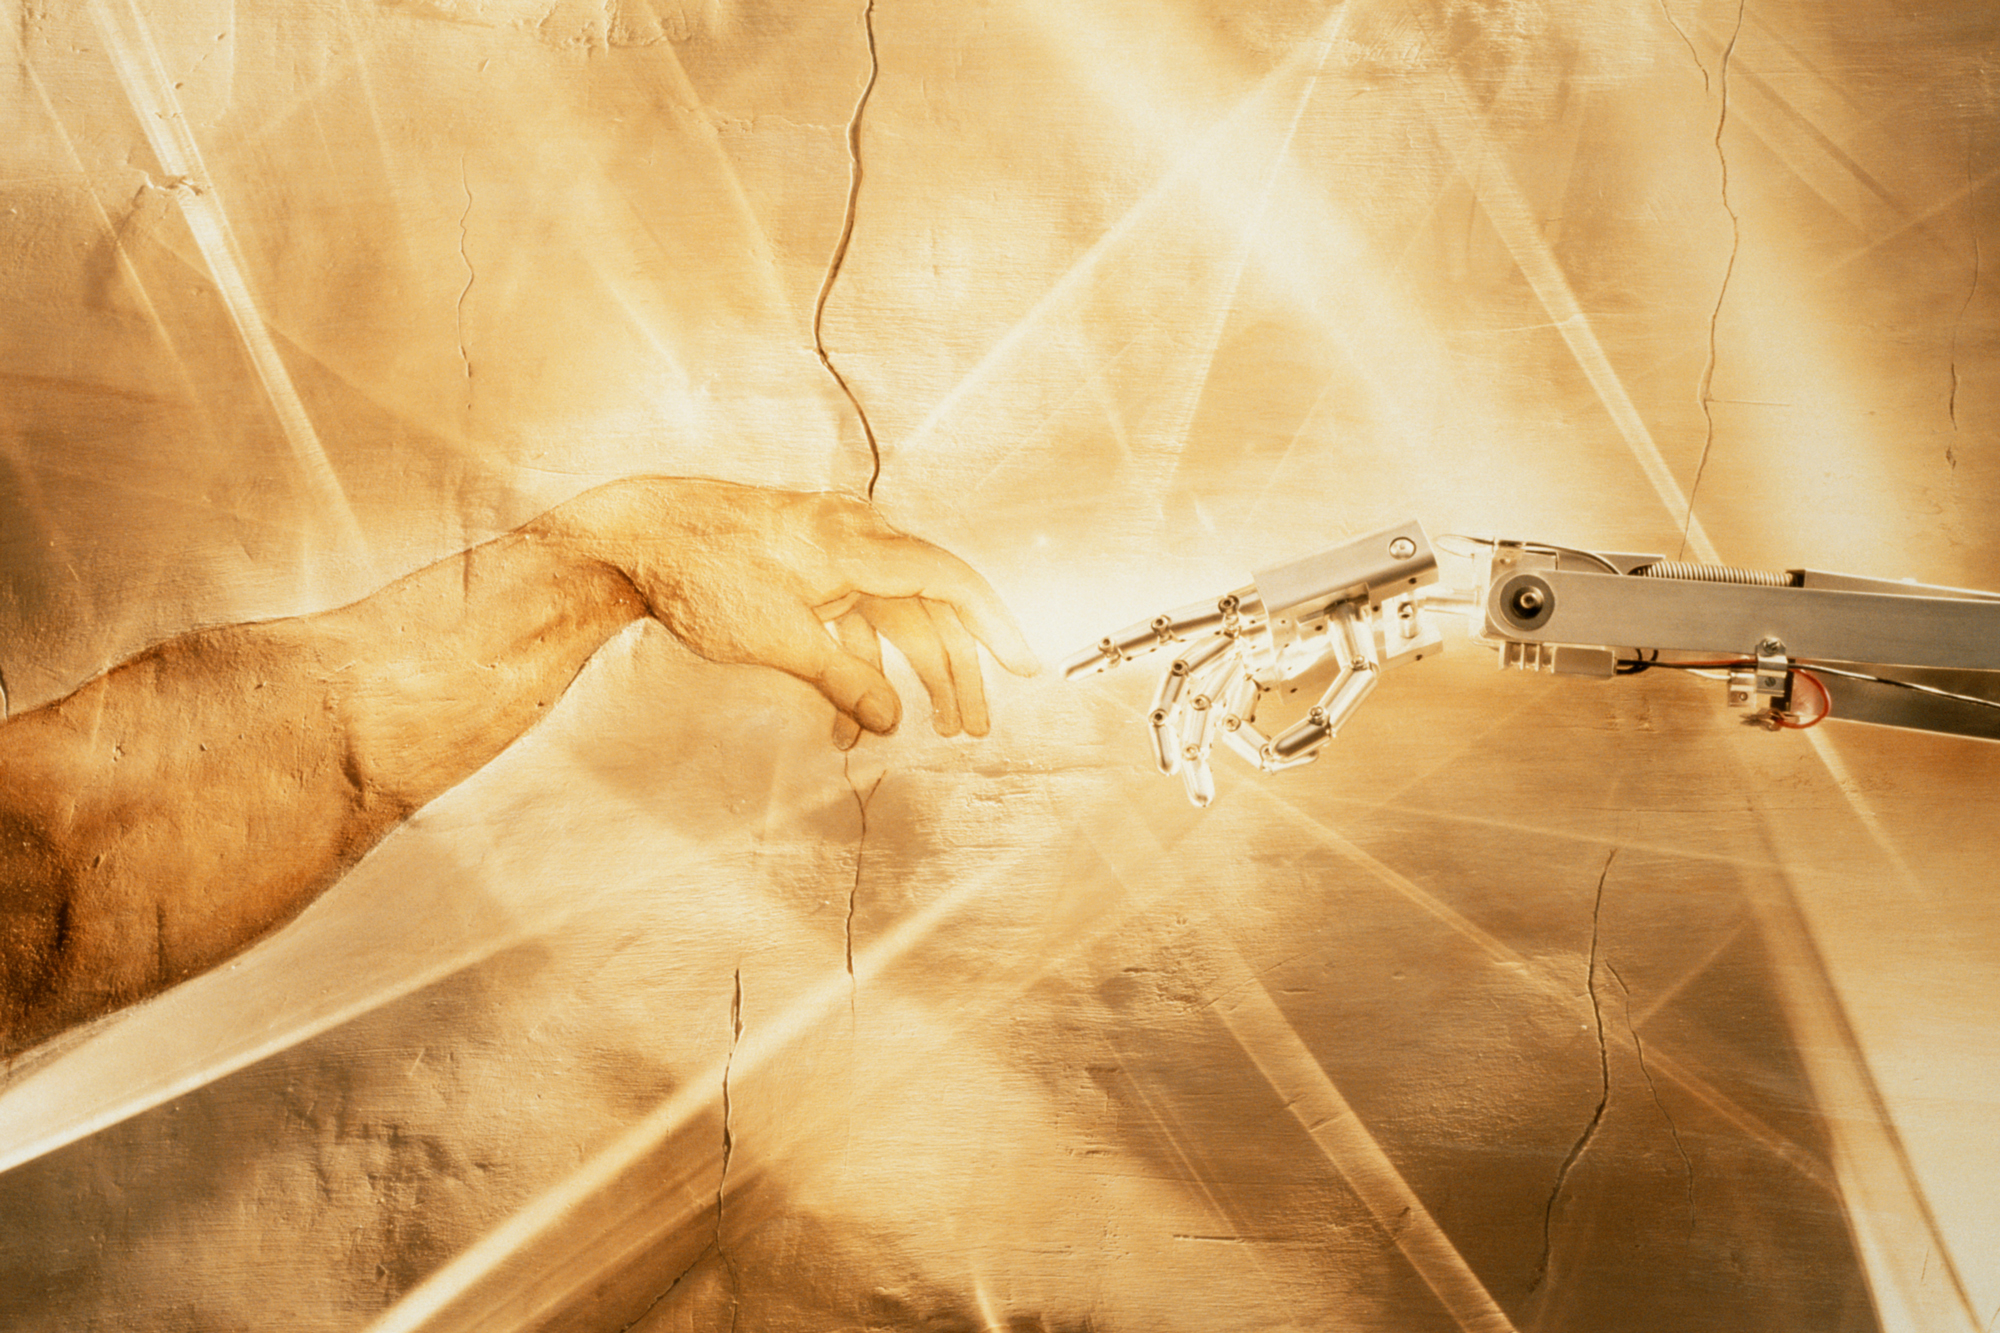
\includegraphics[height=\paperheight]{../img/hands-touch-of-god.jpg}
    }
    \maketitle
  }

  \begin{frame}{The Outline}
    \tableofcontents
  \end{frame}

%%%%%%%%%%%%%%%%%%%%%%%%%%%%%%%%%%%%%%%%%%%%%%%%%%%%%%%%%%%%%%%%%%%%%%%%%%%%%%%%

  \section{General AI: One Summer Dream}

%%%%%%%%%%%%%%%%%%%%%%%%%%%%%%%%%%%%%%%%%%%%%%%%%%%%%%%%%%%%%%%%%%%%%%%%%%%%%%%%

  \section{AI in Games}
  \begin{frame}[standout]
    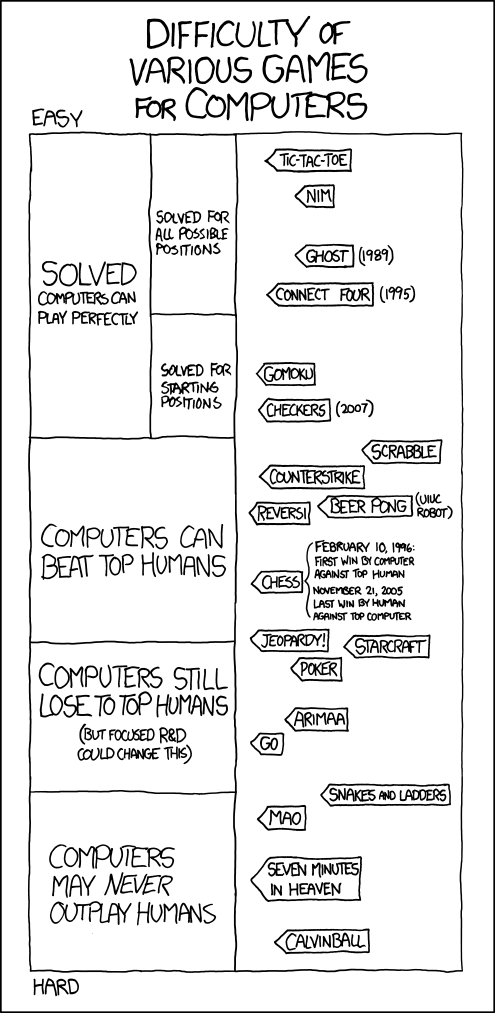
\includegraphics[height=\paperheight]{../img/game_AIs.png}
    \nocite{xkcdGameAIs}
  \end{frame}

%%%%%%%%%%%%%%%%%%%%%%%%%%%%%%%%%%%%%%%%%%%%%%%%%%%%%%%%%%%%%%%%%%%%%%%%%%%%%%%%

  \section{Chess: Deep Blue}

%%%%%%%%%%%%%%%%%%%%%%%%%%%%%%%%%%%%%%%%%%%%%%%%%%%%%%%%%%%%%%%%%%%%%%%%%%%%%%%%

  \section{Jeopardy!: Watson}

%%%%%%%%%%%%%%%%%%%%%%%%%%%%%%%%%%%%%%%%%%%%%%%%%%%%%%%%%%%%%%%%%%%%%%%%%%%%%%%%

  \section{Atari Games:\\
    Deep Reinforcement Learning}
  {
    \setbeamertemplate{frame footer}{\atariCitation}
    \begin{frame}{Atari Player by Google DeepMind}
      \begin{center}
        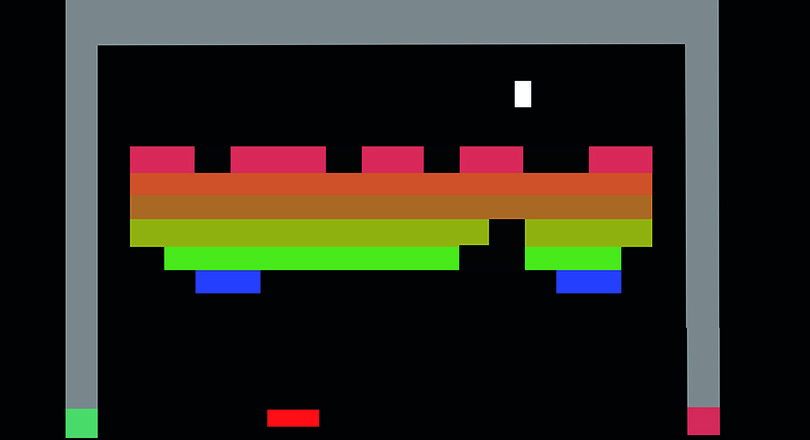
\includegraphics[width=\textwidth, height=\textheight, keepaspectratio]{../img/atari_breakout.jpg}

        \url{https://youtu.be/0X-NdPtFKq0?t=21m13s}
      \end{center}
    \end{frame}
  }

  {
    \setbeamertemplate{frame footer}{\url{https://youtu.be/0X-NdPtFKq0?t=16m57s}}
    \begin{frame}{Reinforcement Learning}
      \begin{center}
        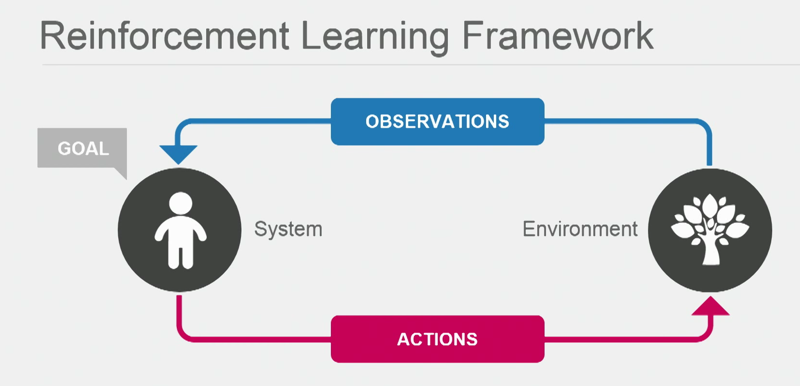
\includegraphics[width=\textwidth]{../img/RL_framework.png}
      \end{center}
      \pause
      games of \textbf{self-play}
    \end{frame}
  }

%%%%%%%%%%%%%%%%%%%%%%%%%%%%%%%%%%%%%%%%%%%%%%%%%%%%%%%%%%%%%%%%%%%%%%%%%%%%%%%%

  \section{Go:\\
    AlphaGo, AlphaGo Zero, AlphaZero}
  {
    \setbeamertemplate{frame footer}{\alphaGoCitation}
    \begin{frame}{Tree Search}
      Optimal value~$v^*(s)$ determines the~outcome of~the game:
      \pause
      \begin{itemize}[<+- | alert@+>]
          \tiny
        \item from every board position or state $s$
        \item under perfect play by~all players.
      \end{itemize}
      \pause

      It is computed by~\textbf{recursively traversing a~search tree} containing approximately $b^d$ possible sequences of moves, where
      \pause
      \begin{itemize}[<+- | alert@+>]
          \tiny
        \item $b$ is the game’s breadth (number of legal moves per position)
        \item $d$ is its depth (game length)
      \end{itemize}
    \end{frame}
  }

  {
    \setbeamertemplate{frame footer}{\cite{Allis1994searching}}
    \begin{frame}{Game tree of~Go}
      Sizes of~trees for~various games:
      \begin{itemize}
        \item chess: $b \approx 35, d \approx 80$
        \item Go: $b \approx 250, d \approx 150$
          \pause
          $\Rightarrow$ more positions than atoms in the universe!
      \end{itemize}
      \pause

      \epigraph{
        That makes Go a \textbf{googol} times more complex than chess.
      }{\tiny\url{https://deepmind.com/alpha-go.html}}
      \pause

      \vskip -1em
      How to handle the size~of the game tree?
      \pause
      \begin{itemize}[<+- | alert@+>]
        \item for the breadth: a~neural network to~select moves
        \item for the depth: a~neural network to~evaluate current position
        \item for the tree traverse: Monte Carlo tree search (MCTS)
      \end{itemize}
    \end{frame}
  }

  \begin{frame}{Monte Carlo tree search}
    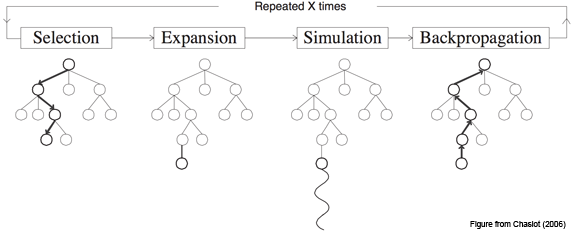
\includegraphics[width=\textwidth]{../img/MCTS.png}
  \end{frame}

%%%%%%%%%%%%%%%%%%%%%%%%%%%%%%%%%%%%%%%%%%%%%%%%%%%%%%%%%%%%%%%%%%%%%%%%%%%%%%%%

  \section{Poker: Cepheus, DeepStack}
  {
    \setbeamertemplate{frame footer}{\cepheusCitation}
    \begin{frame}{Cepheus\\
        \tiny Heads-up Limit Hold’em Poker}
      \pause
      \begin{center}
        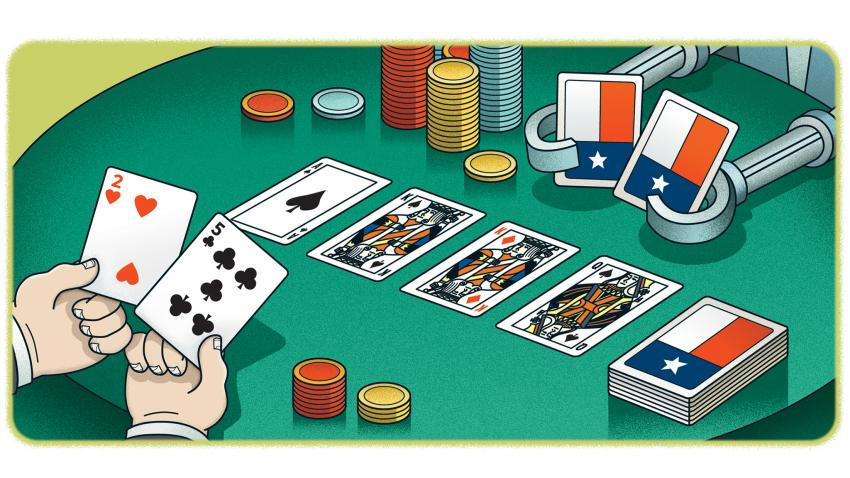
\includegraphics[width=\textwidth, keepaspectratio]{../img/limit_holdem_poker.jpg}

        \url{http://poker.srv.ualberta.ca/}
      \end{center}
    \end{frame}
  }


%%%%%%%%%%%%%%%%%%%%%%%%%%%%%%%%%%%%%%%%%%%%%%%%%%%%%%%%%%%%%%%%%%%%%%%%%%%%%%%%

  \section{Beyond DeepStack: TensorCFR}

%%%%%%%%%%%%%%%%%%%%%%%%%%%%%%%%%%%%%%%%%%%%%%%%%%%%%%%%%%%%%%%%%%%%%%%%%%%%%%%%

  \section{Conclusion}

  \begin{frame}[standout]
    \begin{center}
      Thank you!

      Questions?
    \end{center}
  \end{frame}

%%%%%%%%%%%%%%%%%%%%%%%%%%%%%%%%%%%%%%%%%%%%%%%%%%%%%%%%%%%%%%%%%%%%%%%%%%%%%%%%

  \appendix
  \begin{frame}[standout]
    Backup Slides
  \end{frame}

  % TODO display (I), (II) instead of i, ii
  \begin{frame}[allowframebreaks]{Further Reading}
    \tiny
    % TODO fill in relevant Further Reading
    % Machine Learning:
    % \begin{itemize}
    %   \item \textbf{Deep Learning} (\cite{Lecun2015deep})
    %   \item \textbf{Deep Learning course} \url{https://www.udacity.com/course/deep-learning--ud730}
    % \end{itemize}
  \end{frame}

  \begin{frame}[allowframebreaks]{References}
    \tiny
    \printbibliography[heading=none]
  \end{frame}

\end{document}
